\chapter{Transition Plugins}%
\label{cha:transition_plugin}

When playing a section of media where one edit ends and another edit begins on the timeline,
the usual result is that the first edit's output immediately is followed by the second edit.  Transitions provide a better method whereby the first edit’s output becomes the second edit’s output.  There are several different audio and video transitions listed in the Resources window as figure~\ref{fig:transition}.

\begin{figure}[htpb]
    \centering
    \includegraphics[width=0.8\linewidth]{transition.png}
    \caption{Resources window displaying the Video Transitions.}
    \label{fig:transition}
\end{figure}

Note the colored bar above the \textit{Shape Wipe} transition.
This bar near the transition symbol shows the position and the length of the transition.

Transitions only apply to the matching track type; that is audio transitions only apply to audio tracks
and video transitions only apply to video tracks.

An example usage of a transition follows:
\begin{enumerate}
    \item Load a single video file and delete a sizable section from within the video which will result in two edits of that file. Now you should see the edit boundary between the two edits on the timeline.
    \item Move to the \textit{Resources window} and click on the \textit{Video transitions} folder. Choose a transition by highlighting it and then drag and drop it on the second video edit on the timeline. A colored box shows where the transition will appear and when you release the mouse the $2^{nd}$ edit applies the transition between the $1^{st}$ and $2^{nd}$ edit.
The beginning of the edit will be covered by the transition, if the insertion point or the In point is over an edit.
\end{enumerate}
Some Transitions have parameters that can be modified. To see these, move the pointer over the transition and right click which brings up a menu. A \texttt{Show} option will pop up a window if there are parameters that you can change to different values. 
An \textit{On} option makes it possible to turn off the transition so that it will not be in effect in case you want to only enable it under certain conditions.  The default value for this will be checked On.
A \textit{Length} option lets you adjust the length in seconds of the time that the transition will be in play.  Values modified in the Show or Length will be saved for use the next time that transition is used until changed again. 
The \textit{Detach} option deletes the transition from the timeline. When you drag and drop a different transition on top of an existing transition on the timeline, it replaces the previous one.

There are some shortcuts to alleviate the dragging and dropping of transitions when you want to do a lot of them in various places on the timeline. After you have established the parameter values for a transition that you have dragged from the Resources window, you can use "U" and "u" keys to paste the same transition;
the "U" key pastes the last video transition while the "u" key pastes the last audio transition on all recordable tracks. 
Alternatively, you can add the same transition to multiple edits when in \textit{Arrow mode} (Drag and Drop editing), by selecting edits to add the transition to and use the Video/Audio pulldown to \textit{Attach transition}. Select the desired transition and then click the checkmark OK. You can set a default transition in the Attach transition popup box -- by highlighting your choice, then click on the button \textit{Set Default Transition}, and you will see that transition become the new default.

The way that transitions work is that two edits overlap for some length of time and no edits are actually moved during the transitions.
Instead extra frames from the source file will be used to lengthen the first edit enough to make it overlap the second edit for the length of the transition. The transition takes effect exactly at the beginning of the second edit and lasts for the specific length of time you set into the second edit. 
What this means is that if you set a duration of 2 seconds for a flash transition, it will not start at the last 1 second of the first edit and continue 1 second into the second edit. Instead the transition will start exactly at the beginning of the second edit and last for 2 seconds into that second edit. 
This is why it is necessary that the first edit needs to have extra data after the end boundary to provide enough fill for the transition length into the second edit.
In the case where the last frame on the timeline is the last frame of the source, \CGG{} will lengthen the first edit using only that last frame.  The result will not be what you want because the first edit will freeze into the transition.

When playing transitions, software rendering is used.  This means that if you are using hardware, as with the video driver set to OpenGL, hardware acceleration will usually be turned \textit{off} during the transition and \textit{on} after the transition. Consequently, you may notice small anomalies while playing this section but you can avoid this by switching to using X11 video driver instead or just ignore it because when you create your final render that is always done in software only.
    
When \textit{Info on} is enabled via the right mouse button over an empty space in the Resources window (or the shortcut of the letter “i” is used), a short description will be provided in the lower right hand corner of that window for the current transition that the mouse is on.

Once you have dragged and dropped a transition to the timeline, right mouse click on the transition and a pop-up menu will appear which provides an opportunity to make some changes.  These are described next for all video and audio transitions. 

\begin{description}
    \item[Show] If available, clicking on this will pop up a transition specific menu.
    \item[On] Toggle on/off the transition effect so that you can see what it looks like when played. Ordinarily this will be checked to indicate it is On.
    \item[Transition length] When you click on Length, a pop-up menu will come up.  Set the length in seconds, frames, samples, \textit{H:M:S:frm} or \textit{H:M:S.xxx} for the transition to complete either by typing a value into the text box or using the tumbler arrows.  In addition you can use the mouse wheel to change the length in real time. You will see the colored bar get longer or shorter as you change the length. 
There is a down arrow next to the Seconds box allowing for changing to the other dimensions of frames, samples, etc.  The mathematics is automatically done for you to convert it to seconds if not already in that dimension.
    \item[Detach] Remove the transition from the timeline.
\end{description}

\section{Audio Transitions}%
\label{sec:audio_transition}

\subsection*{Crossfade}%
\label{sub:crossfade}

Creates a smooth transition from one audio source edit to another. The crossfade has the first source \textit{fade out} while the second \textit{fades in}.

\section{Video Transitions}%
\label{sec:video_transition}

\subsection*{BandSlide}%
\label{sub:bandslide}

Bands slide across video and you see the image slide.

\subsection*{BandWipe}%
\label{sub:bandwipe}

Bands wipe across the video and you see the mask slides.

\subsection*{Dissolve}%
\label{sub:dissolve}

A soft dissolve where the In segment becomes more transparent while the Out segment begins to gradually show in its place until fully there.

\subsection*{Flash}%
\label{sub:flash}

The video flashes when transitioning between segments.

\subsection*{IrisSquare}%
\label{sub:irissquare}

Video switches segments via a small rectangular view that gradually grows to full size.

\subsection*{Shape Wipe}%
\label{sub:shape_wipe}

Wipe a specific shape across the video. Currently available 63 shapes are:

\begin{center}
	\begin{longtable}{p{4cm}p{4cm}p{4cm}}
		\label{tabular:transitions}
		\textit{asimetric\_clocks} & \textit{asimetric\_clocks\_2} & \textit{audio} \\
		\textit{burst} & \textit{Butterfly} & \textit{Circle-h\_01} \\
		\textit{Circle-h\_02} & \textit{Circle-v\_01} & \textit{Circle-v\_02} \\
		\textit{circle} & \textit{clock} & \textit{Clouds\_01} \\
		\textit{Clouds\_02} & \textit{crazy\_clock} & \textit{cream} \\
		\textit{Cross-Iris\_01} & \textit{Cross\_01} & \textit{Diagonal-Curve} \\
		\textit{Diagonal-Linear} & \textit{Diamond-Iris\_01} & \textit{Diamond\_01} \\
		\textit{Diamond\_02} & \textit{Diamond\_03} & \textit{Double-Door-h} \\
		\textit{Double-Door-v} & \textit{film} & \textit{film2} \\
		\textit{Gravity} & \textit{heart} & \textit{Linear-h} \\
		\textit{Linear-v} & \textit{mosaic} & \textit{multi\_box} \\
		\textit{Plasma\_01} & \textit{rare\_spiral} & \textit{specks} \\
		\textit{spiral} & \textit{spiral\_clock} & \textit{square} \\
		\textit{squares} & \textit{star} & \textit{tile2x2h} \\
		\textit{tile2x2v} & \textit{Venetian-Blinds-h-x05} & \textit{Venetian-Blinds-h-x10} \\
		\textit{Venetian-Blinds-v-x05} & \textit{Venetian-Blinds-v-x10} & \textit{water} \\
\\
                \textit{Cinelerra16-9-Heavy} & \textit{Cinelerra16-9-Light} & \textit{CinelerraGG} \\
                \textit{16-9\_boart} & \textit{16-9\_boxes} & \textit{16-9\_cat\_eyes} \\
                \textit{16-9\_film\_bands} & \textit{16-9\_multi\_circle} & \textit{16-9\_multi\_spiral} \\
                \textit{16-9\_multi\_square} & \textit{16-9\_rare\_spiral} & \textit{16-9\_rectangles} \\
                \textit{16-9\_star} & \textit{16-9\_stars} & \textit{16-9\_wood} \\

		\bottomrule
	\end{longtable}
\end{center}
The menu for Shape Wipe that popups when you click on \textit{Show} has several possible choices.  First, the \textit{Shape} allows for choosing from the list of shapes as outlined previously either by typing in the textbox, using the down arrow, or clicking on the tumbler down/up arrows.
Next, there is a \textit{Feather} textbox with tumbler arrows or a slider bar to easily change the blending amount.  A reset button is conveniently located to the right of the slider bar.  There is a checkbox to \textit{Preserve shape aspect ratio} and a \textit{Direction} of \textit{White to Black} or \textit{Black to White} (figure~\ref{fig:star}).

\begin{figure}[htpb] \centering
	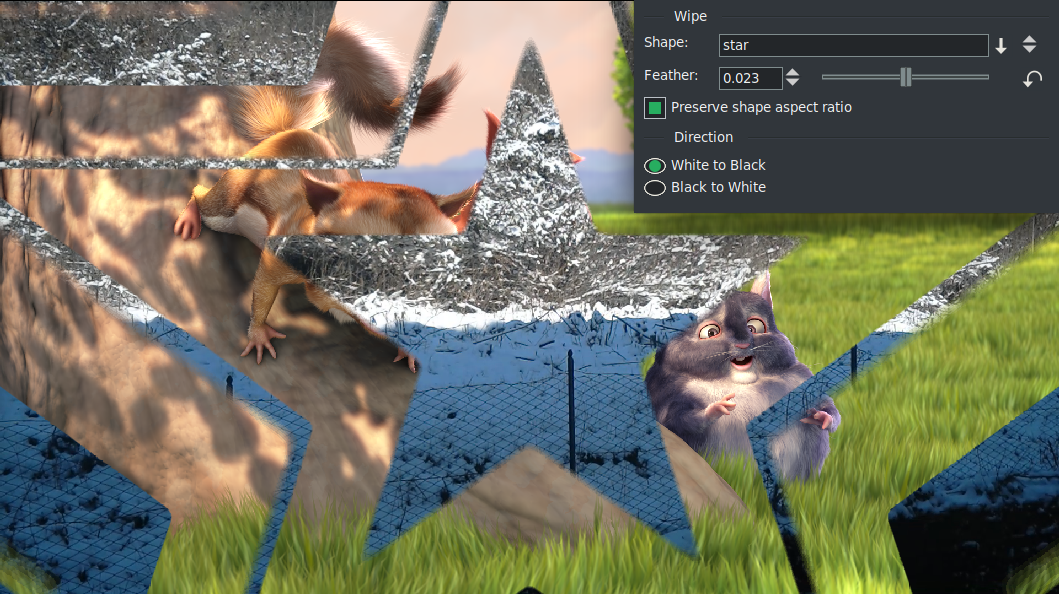
\includegraphics[width=0.9\linewidth]{star.png}
	\caption{Example of the Shape Wipe $\rightarrow$ Star}
	\label{fig:star}
\end{figure}

You can add your own images to the Shape Wipe transition and there are some free ones available to download such as under the \texttt{Video $\rightarrow$ Transitions} pulldown at {\small \url{http://assistcg.com}}.

To include new images in the Shape Wipe Transition, simply copy the file \textit{shape.jpg} or
\textit{shape.png} to the subdirectory \texttt{plugins/shapes} in your \CGG{} directory path. If
you prefer to have a better quality png used instead of the included 90\% jpg version, you can download
the equivalent png versions at {\small \url{https://cinelerra-gg.org/download/ShapeWipe\_pngs.txz}}.
You will then need to untar this file, choose the ones you want, and add them to your directory path.
After an update of \CGG{}, they will have to be restored each time.

\subsection*{Slide}%
\label{sub:slide}

Image slides into view; you can set Left/Right/In/Out.

\subsection*{Wipe}%
\label{sub:wipe}

Wipe the image across screen starting left or right.

\subsection*{Zoom}%
\label{sub:zoom}

Zoom out video at $\frac{X}{Y}$ magnification for some seconds.

